\documentclass{article}
\usepackage{amsmath}
\usepackage{amsthm}
\usepackage{enumerate}
\usepackage[bookmarks=true]{hyperref}
\usepackage{bookmark}
\usepackage{graphicx}
\usepackage{multirow}
\usepackage{adjustbox}
\usepackage{wrapfig}
\usepackage{subcaption}
\usepackage{color}
\usepackage[dvipsnames]{xcolor}

\usepackage{amssymb,amsmath,amsthm,amsfonts}
\usepackage{mathrsfs}
\usepackage{dsfont}
\usepackage{enumerate}

%% \newtheorem{mdef}{Definition}

\newcommand{\eqsplit}[2]{
  \begin{equation}\label{#2}
    \begin{split}
      #1
    \end{split}
  \end{equation}}
\newcommand{\eqnsplit}[1]{
  \begin{eqnarray*}
    #1
  \end{eqnarray*}}
\newcommand{\tran}[1]{
  \tilde{#1}
}
\newcommand{\td}[2]{
  \frac{d #1}{d #2}
}
\newcommand{\pd}[2]{
  \frac{\partial #1}{\partial #2}
}
\newcommand{\ppd}[2]{
  \frac{\partial^2 #1}{\partial #2^2}
}
\newcommand{\pdd}[3]{
  \frac{\partial^2 #1}{\partial #2 \partial #3}
}
\newcommand{\otd}[1]{
  \frac{d}{d #1}
}
\newcommand{\opd}[1]{
  \frac{\partial}{\partial #1}
}
\newcommand{\oppd}[1]{
  \frac{\partial^2}{\partial #1^2}
}
\newcommand{\opdd}[2]{
  \frac{\partial^2}{\partial #1 \partial #2}
}
\newcommand{\ket}[1]{
  |#1\rangle
}
\newcommand{\bra}[1]{
  \langle#1|
}
\newcommand{\inn}[1]{
  \langle#1\rangle
}
\newcommand{\mean}[1]{
  \langle#1\rangle
}
\newcommand{\tr}{
  \text{tr}\,
}
\newcommand{\re}{
  \text{Re}\,
}
\newcommand\im{
  \text{Im}\,
}
\newcommand{\arcsinh}{
  \sinh^{-1}
}
\newcommand{\arccosh}{
  \cosh^{-1}
}
\newcommand{\erfc}{
  \text{erfc}
}
\newcommand{\E}{
  \mathbb{E}
}
\renewcommand{\P}{
  \mathbb{P}
}
\newcommand{\I}{
  \mathbf{1}
}
\newcommand{\1}[1]{
  \mathbf{1}_{\{#1\}}
}
\newcommand{\diag}{
  \text{diag\,}
}
\newcommand{\pop}[1]{
\varepsilon_{#1}
}

\newcommand{\M}{
  {\text{max}}
}
\newcommand{\m}{
  {\text{min}}
}
% \newcommand{\ph}{
%   {\text{arg}\,}
% }
\newcommand\erf{
  \text{erf}
}
\renewcommand\vec[1]{
  \mathbf{#1}
}
\newcommand\cov{
  \text{cov}
}
\newcommand\var{
  \text{var}
}
\newcommand\cor{
  \text{cor}
}
\DeclareMathOperator*{\argmin}{argmin}
\DeclareMathOperator*{\argmax}{argmax}
\newcommand\mtx[1]{
  \mathbf{#1}
}
\renewcommand \L {
  \mathfrak{leb}
}
\newcommand{\hot}{
  \text{h.o.t.}
}


%% \newtheorem{proposition}{Proposition}
\newtheorem{theorem}{Theorem}
\newtheorem{acknowledgement}{Acknowledgement}
\newtheorem{algorithm}{Algorithm}
\newtheorem{axiom}{Axiom}
\newtheorem{case}{Case}
\newtheorem{claim}{Claim}
\newtheorem{conclusion}{Conclusion}
\newtheorem{condition}{Condition}
\newtheorem{conjecture}{Conjecture}
\newtheorem{corollary}{Corollary}
\newtheorem{criterion}{Criterion}
\newtheorem{definition}{Definition}
\newtheorem{example}{Example}
\newtheorem{exercise}{Exercise}
\newtheorem{lemma}{Lemma}
\newtheorem{notation}{Notation}
\newtheorem{problem}{Problem}
\newtheorem{proposition}{Proposition}
\newtheorem{remark}{Remark}
\newtheorem{solution}{Solution}
\newtheorem{summary}{Summary}

\title{Tail Indices and Scale Parameters in Financial Time Series}
\author{Thomas Mikosch, Casper de Vries, Xie Xiaolei}
\date{\today}
\begin{document}
\maketitle

\begin{abstract}
We consider an investor with preferences that accord with Generalized
Disappointment Aversion. Such an investor cares about downside risk and
we assume he recognizes the heavy tail feature of asset return
distributions. We argue that when a market is dominated by rational
investors of this kind, the return distributions of equities that are
actively traded in this market must have very similar tail indices. We
also show, in contrast, the scale parameters of the return
distributions may differ hugely from one another.

On the other hand, whether or not all equities in a multivariate model
have the same tail index is a dividing issue for multivariate GARCH
models proposed in the literature. Therefore, it is important to analyze
data of real equity returns and see how close to each other the
tail indices actually are.

In this work empirical results are also presented and they appear
to support the conclusion that the tail indices are very similar,
with respect to the confidence bands of estimation.
\end{abstract}

\section{Introduction}
It is generally believed that the utility function of an
investor is increasing and concave -- as John H. Cochrane
put it, ``the last bite is never as satisfying as the first''
\cite{cochrane2009asset}. This implies investors are considerably
more concerned about large losses than are cheered by large gains.
Furthermore, it is a stylized fact that equity return distributions
are heavy-tailed (see e.g. Jansen and de Vries \cite{jansen1991frequency}).
In particular, the lower-tail of an equity distribution is often heavier
than the upper-tail of the same distribution.

We show in this paper that concerns of the down-side risk and the
heavy-tail property of equity returns  imply that the lower-tail indices
of actively traded equities in a rational market must be fairly close to
one another.

%% A cornerstone of this conclusion is the empirical fact that equity
%% return distributions are heavy-tailed (see e.g. Jansen and de Vries
%% (1991) \cite{jansen1991frequency}). If investors and speculators alike
%% display concern for downside risk, as formulated via a utility function,
%% it is important to model this risk adequately. 

In section \ref{sec:GDA}, we explicitly recognize the behavioral
concern for downside risk in the investor's evaluation of portfolios
using the framework of Generalized Disappointment Aversion (GDA)
introduced by Routledge and Zin \cite{routledge2010generalized}. GDA
is an extension of the concept of Disappointment Aversion (DA) of Gul
(1991) \cite{gul1991theory}. The Gul paper derives the DA from first
principles (axiomatic).

%% Secondly, the empirical fact that the loss return distribution is
%% non-normally fat tailed distributed is taken into account.
%% If investors and speculators alike display concern for downside risk,
%% as formulated by a utility function, it becomes important to model this 
%% risk adequately. see e.g. Jansen and de Vries (1991), exhibiting power
%% like tails rather than exponential tails. The risk is determined both
%% by the coefficient that regulates the hyperbolic power and the
%% scale. We reason how both determine the risk of investment apart from
%% the mean return.

%% \section{Notations}
%% Here is a summary of the notations that we use in the rest of the paper.
%% In this summary $x_F$ denotes a quantity whose value that should be
%% obvious from the context where the notation in question is used.
%% \begin{itemize}
%% \item $\sim$ stands for ``asymptotically equivalent to'', i.e.
%%   $F(x) \sim G(x)$ means
%%   \[
%%   \lim_{x \to x_F} {F(x) \over G(x)} = 1
%%   \]
%% \item $O(F(x))$ stands for terms of the same order as $F(x)$, i.e.
%%   \[
%%   \lim_{x \to x_F } {O(F(x)) \over F(x)} = \text{constant}
%%   \]
%% \item $o(F(x))$ stands for terms of higher orders than $F(x)$, i.e.
%%   \[
%%   \lim_{x \to x_F } {o(F(x)) \over F(x)} = 0
%%   \]
%% \item $\hot$ stands for ``higher order terms'', i.e.
%%   \[
%%   \lim_{x \to x_F} {F(x) + \hot \over F(x)} = 1
%%   \]
%% \end{itemize}

%% \section{Implications of heavy-tailed equity return}
%% \label{sec:1}
%% In this section we consider a rather general utility functional
%% $U(F)$ associated with the distribution function $F(\cdot)$ of
%% an equity return $X$. We define $U(F)$ as
%% \[
%% U(F) = \E u(X)
%% \]
%% for some function $u(\cdot)$ satisfying the following conditions:
%% \begin{enumerate}
%% \item $u(\cdot)$ is defined on $\mathbb R$, is increasing, concave
%%   and differentiable.
%% \item $u(\cdot)$ is independent of the distribution of $X$
%% \item $\lim_{x \to \infty} u(x) = \bar u$, where $\bar u$ is a
%%   constant
%% \end{enumerate}
%% %% An exampple of such utility functions is
%% %% \[
%% %% u(x) = \bar u - e^{-\lambda x}
%% %% \]
%% %% for some $\lambda > 0$.
%% In addition we assume $F(\cdot)$ has the following properties:
%% \begin{enumerate}
%% \item $\lim_{x \to -\infty} F(x) u(x) = 0$
%% \item $\lim_{x \to -\infty} {|x|^\alpha F(x) \over L(|x|)} = 1$
%% \item $\lim_{x \to \infty} {x^\alpha (1 - F(x)) \over L(x)} = 1$
%% \end{enumerate}
%% for some $\alpha > 1$ and some slowly varying function $L(x) > 0$
%% defined on $\mathbb R_+$.
%% $\E u(X)$ can be computed as follows
%% \begin{eqnarray*}
%%   && \E u(X) \\
%%   &=& \int_{-\infty}^{\infty} u(x) d F(x) \\
%%   &=& \left. u(x) F(x) \right|_{-\infty}^{\infty}
%%   - \int_{-\infty}^\infty F(x) u'(x) dx \\
%%   &=& \bar u - \left(
%%   \int_{-\infty}^{-M} + \int_{-M}^{M} + \int_{M}^{\infty}
%%   \right) F(x) u'(x) dx
%% \end{eqnarray*}
%% As $M \to \infty$ we have for the lower-tail integral
%% \begin{eqnarray*}
%%   && \int_{-\infty}^{-M} F(x) u'(x) dx \\
%%   &\sim& \int_{-\infty}^{-M} L(|x|) |x|^{-\alpha} u'(x) dx \\
%%   &=& \int_{M}^{\infty} L(x) x^{-\alpha} u'(-x) dx \\
%% \end{eqnarray*}
%% Applying the same calculation to the upper-tail integral and
%% using $1 - F(x) \sim L(x) x^{-\alpha}$ yields
%% \begin{eqnarray}
%%   && \E u(X) \nonumber \\
%%   &=& \bar u - \int_{M}^\infty L(x) x^{-\alpha} u'(-x) dx
%%   -\int_{-M}^M F(x) u'(x) dx \nonumber \\
%%   && -\int_{M}^\infty [1 - L(x) x^{-\alpha}] u'(x) dx
%%   + \hot \nonumber \\
%%   &=& u(M) - \int_{M}^\infty L(x) x^{-\alpha} [u'(-x) - u'(x)] dx
%%   + \hot \nonumber \\
%%   && - \int_{-M}^M F(x) u'(x) dx \label{eq:xxie0}
%% \end{eqnarray}
%% In the simple case where $L(x) = A$, i.e. a constant, we have
%% \begin{eqnarray}
%%   \pd{\E u(X)}{\alpha} &=& \int_M^{\infty} A x^{-\alpha} \ln(x)
%%      [u'(-x) - u'(x)] dx +\hot \nonumber \\
%%      \pd{\E u(X)}{A} &=& -\int_M^{\infty} x^{-\alpha} [u'(-x) - u'(x)] dx
%%      + \hot
%%   \label{eq:xxie01}   
%% \end{eqnarray}
%% By concavity $u'(-x) > u'(x)$ for $x \in (M, \infty)$. So for large
%% $M$,
%% \[
%% \pd{\E u(X)}{\alpha} > 0, \quad \pd{\E u(X)}{A} < 0
%% \]
%% %% \begin{eqnarray*}
%% %%   \pd{\E u(X)}{\alpha} &>& 0 \\
%% %%   \pd{\E u(X)}{A} &<& 0
%% %% \end{eqnarray*}
%% Now that each and every equity is assigned a score by the utility
%% functional, all equities actively traded in a rational market that
%% is dominated by agents exhibiting a utility function must have almost
%% equal scores -- otherwise trading will be concentrated on those
%% with top scores.

%% Suppose the equity with the highest score in the market has parameters
%% $(\alpha, A)$. We would like to find out how these parameters vary across
%% equities that score almost as high. Consider a parameter pair
%% $(\alpha + \Delta \alpha, A + \Delta A)$. If it scores the same as
%% $(\alpha, A)$, we have
%% \[
%% 0 = \Delta \E u(X) = \Delta \alpha \pd{\E u(X)}{\alpha}
%% + \Delta A \pd{\E u(X)}{A} + \hot
%% \]
%% Discarding higher order terms and plugging \eqref{eq:xxie01} into
%% this equation gives
%% \[
%%   {\Delta \alpha \over \Delta A}
%%   =
%%   {
%%     \int_M^{\infty} x^{-\alpha} [u'(-x) - u'(x)] dx    
%%     \over
%%     \int_M^{\infty} A x^{-\alpha} \ln(x) [u'(-x) - u'(x)] dx    
%%   }
%% \]
%% Taking the limit as $M \to \infty$, we get
%% \[
%% \lim_{M \to \infty} {\Delta \alpha \over \Delta A}
%% =
%% \lim_{M \to \infty} {1 \over A \ln(M)} = 0
%% \]
%% We see from the last equation that in the configuration space around
%% $(\alpha, A)$, a small variation of $\alpha$ induces a tremendous
%% variation of $A$. Furthermore, this conclusion does not depend on the
%% choice of the function $u(\cdot)$. Thus in a market dominated by rational
%% agents guided by their utility functionals, we can expect to see very
%% similar tail indices but hugely different scale parameters in equity
%% return distributions.

%% %% Due to concavity, $u'(-x) > u'(x)$ on the interval $(M, \infty)$.
%% %% The central region integral on $(-M, M)$ does not depend on $\alpha$.
%% %% So $\E u(X)$ is monotonically increasing with $\alpha$. Trying to
%% %% maximize his utility function, an agent will seek the largest $\alpha$
%% %% possible in the market. As a result, all equities traded with significant
%% %% volumes must eventually become so close that they are indistinguishable
%% %% by available statistical methods.

%% In section \ref{sec:GDA}, we compute the utility function within the
%% elaborate framework of {\it Generalized Disappointment Aversion} and
%% show that the same conclusion stands -- tail indices are similar while
%% scale parameters can be drastically different.

\section{Generalized disappointment aversion}
\label{sec:GDA}
Routledge and Zin (2010) \cite{routledge2010generalized} define the GDA
preferences over discrete states in their formula (2). A slight extension
is to consider a continuum of possible states. Suppose the state variable
$C$ is continuously supported on $(0, \infty)$ and has distribution
function $G(\cdot)$. The utility function of an agent exhibiting GDA
preferences reads
\begin{equation}
  u(v)= \E u(C) - b \int_{0}^{\delta v}
  \left[ u(\delta v) - u(x) \right] dG(x)\label{11}%
\end{equation}
where $\delta > 0$, and $v>0$. Equivalently
\begin{equation}
  \label{eq:xxie0}
  u(v) = \E u(C) - b \E[u(\delta v) - u(C); C < \delta v]
\end{equation}
Here $v$ can be thought of as the certainty payoff equivalent to the
risky payoff $C$. Note that when $b=0$, 
preferences are expected utility; when $\delta=1$ and $b>0$,
preferences follow Gul's (1991) original disappointment aversion.
An agent guided by this utility function will seek to maximize $u(v)$.

\subsection{power-law utility function}
In this section we follow Routledge and Zin
\cite{routledge2010generalized} and assume 
that the utility function of consumption $C$ is a power function%
\begin{equation}
  \label{eq:power_utility}
  u(C)=\frac{1}{1-\gamma}C^{1-\gamma}%  
\end{equation}
where $\gamma > 0$. For simplicity we assume the investor
initially has one unit of wealth. Let $r > 0$ be the return on the
risk free state bond and $X$ be the return on equity. Portfolio weights
are $\left(1-\phi\right)$ and $\phi$ respectively. Then
\begin{equation}
  \label{eq:xxie1}
  %% u(C)=\frac{1}{1-\gamma}V^{1-\gamma} \max \left\{
  %% 0, 1 + (1-\phi) r  +\phi X
  %% \right\}^{1-\gamma} \label{3}%
  C = (1 - \phi) e^r + \phi e^X
\end{equation}

%% \subsubsection[in case gamma > 1]{in case $\gamma > 1$}

\subsubsection[in case gamma > 1]{in case $\gamma > 1$}
In this section we consider power utility functions of
\eqref{eq:power_utility} with $\gamma > 1$. For convenience,
let $\xi = \gamma - 1$. In this case, we assume the following
distribution function $F(\cdot)$ of the equity return:
\begin{equation}
  \label{eq:X_distr}
  F(x) = \left\{
  \begin{array}{ll}
    p \left(
    {K \over K - x}
    \right)^\alpha & x \leq 0 \\
    1 - (1 - p) \left(
    {K' \over K' + x}
    \right)^\beta & x > 0
  \end{array}
  \right.
\end{equation}
Assume $\alpha, \beta > 1$, $0 < p < 1$ and $K > 0$.
Equation
\eqref{eq:xxie0} can be re-arranged as
\begin{eqnarray}
u(v) &=& \E u(C) + b \E [u(C); C < \delta v] - b u(\delta v) \P[C < \delta v] \nonumber \\
&=& \E u(C) + b \E [u(C); C < \delta v] - b u(\delta v) F(q) \label{eq:functional}
\end{eqnarray}
where
\begin{eqnarray*}
  q(r, \phi) &:=& \ln \left( {
    \delta v - (1 - \phi) e^r
    \over
    \phi
} \right) = \ln\left(
e^r + {\delta v - e^r \over \phi}
\right)
\end{eqnarray*}
Note $C < \delta v$ implies
\[
X < q(r, \phi)
\]
Naturally, if an agent invests in a risky asset instead of a riskless
bond, he expects to obtain a higher return from the risky asset than
he is guarranteed from the riskless bond. In our notation,
this means $\delta v > e^r$, which implies $q(r, \phi) > 0$.
The right-hand-side of \eqref{eq:functional} is a functional of the
distribution function of $X$ via \eqref{eq:xxie1}. For convenience
we denote it $\mathcal U(\cdot)$, i.e.
\[
\mathcal U F (\alpha, \beta, K, K', \phi)
= 
\E u(C) + b \E [u(C); C < \delta v] - b u(\delta v) F(q(r, \phi))
\]
Hereafter we abbreviate $q(r, \phi)$ to just $q$. We have
\begin{eqnarray}
  && \mathcal U F (\alpha, \beta, K, K', \phi) \nonumber \\
  &=& \underbrace{
  -{\alpha K^\alpha \over \xi} p
  \int_{-\infty}^0
      {
       1 \over \left[ (1 - \phi) e^r + \phi e^x \right]^{\xi}
      }
  {1 + b \over (K - x)^{\alpha + 1}} dx
  }_{J_1} \nonumber \\
  && -{\beta K'^\beta \over \xi} (1 - p)
  \int_{0}^\infty
  {
   1 \over \left[ (1 - \phi) e^r + \phi e^x \right]^{\xi}
  }
  {1 + b \1{x < q} \over (K' + x)^{\beta + 1}} dx \nonumber \\
  &&
  - b u(\delta v) \left[
    1 - (1 - p) {
      K'^\beta
      \over
      (K' - q)^\beta
    }
  \right]
  \label{eq:xxie1.0}
\end{eqnarray}

\begin{theorem}
  Let
  \[
  G(\alpha, \beta, K, K') =
  \max_{0 < \phi \leq 1} \mathcal U F(\alpha, \beta, K, K', \phi)
  \]
  Let the disappointment threshold $C < \delta v$ be equivalent to $X < -q$. Assume
  \begin{equation}
    \label{eq:xxie1.1}
    K < {
      \alpha e^{1/\alpha} (1 - e^{-r})^\xi
      \over
      (\alpha + 1) A
    }
  \end{equation}
  where
  \[
  A = \max_{x \geq 1} {b x + x^{\alpha + 1} \over b + x^{\alpha + 1}}
  \]
  Then $G(\alpha, \beta, K, K')$ is monotonically increasing with $\alpha$.
\end{theorem}

\begin{proof}
  We show
  \[
  \td{G}{\alpha} > 0
  \]
  Let
  \begin{equation}
    \label{eq:xxie2}
    \hat \phi := \argmax_{0 < \phi \leq 1}
    \mathcal U F(\alpha, \beta, K, K', \phi)
  \end{equation}
  We have
  \[
  G(\alpha, \beta, K, K') = \mathcal U F(\alpha, \beta, K, K', \hat \phi)
  \]
  It follows
  \begin{eqnarray}
    \td{G}{\alpha}
    &=&
    \pd{\mathcal U F}{\alpha}(\alpha, \beta, K, K', \hat \phi)
    + \pd{\mathcal U F}{\phi}(\alpha, \beta, K, K', \hat \phi)
    \pd{\hat \phi}{\alpha}(\alpha, \beta, K, K')
    \label{eq:xxie3}
  \end{eqnarray}
  The definition \eqref{eq:xxie2} implies $\forall \alpha > 1$
  \begin{equation}
    \label{eq:xxie4}
    \pd{\mathcal U F}{\phi}(\alpha, \beta, K, K', \hat \phi) = 0
  \end{equation}
  So the second term of \eqref{eq:xxie3} vanishes. It remains to show
  \begin{eqnarray*}
    \pd{\mathcal U(F)}{\alpha}(\alpha, \beta, K, K', \hat \phi)
    &>& 0
  \end{eqnarray*}
  We have
    \begin{eqnarray*}
      && \pd{\mathcal U(F)}{\alpha}(\alpha, \beta, K, K', \hat \phi) \\
      &=&
      - \frac{\partial}{\partial \alpha} \left\{
        {\alpha p K^\alpha \over \xi} (1 + b)
        \int_{-\infty}^{0}
          \left[
            (1 - \hat\phi) e^r + \hat\phi e^x
          \right]^{-\xi}
          (K - x)^{-\alpha - 1}
        dx \right\} \\
      &=& \underbrace{
        {p \over \xi}
          (1 + b)\int_{0}^{\infty}
        \left[
          (1 - \hat\phi) e^r + \hat\phi e^{-x}
        \right]^{-\xi}
        \ln \left(
          1 + {x \over K}
        \right)
        {\alpha K^{\alpha} dx
          \over
          (K + x)^{\alpha + 1}
        }
      }_{L_1} \\
      && - \underbrace{
        {p \over \xi}
        (1 + b)\int_{0}^{\infty}
        \left[
          (1 - \hat\phi) e^r + \hat\phi e^{-x}
        \right]^{-\xi}
        {K^{\alpha} dx \over (K + x)^{\alpha + 1} }
      }_{L_2}
    \end{eqnarray*}
    Clearly $L_2 < \infty$. For $L_1$, observe
    \begin{eqnarray*}
      L_1 &<&
      {
        \alpha K^\alpha p (1 + b)
        \over
        \xi (1 - \hat\phi)^\xi e^{r \xi}
      }
      \int_0^\infty
      {1 \over (x + K)^{\alpha + 1}}
      \left(1 + {x \over K}\right)
      dx \\
      &=&
      {
        p \alpha (1 + b)
        \over
        \xi (\alpha - 1) (1 - \hat\phi)^\xi e^{r \xi}
      } < \infty
    \end{eqnarray*}
    Let
    \begin{eqnarray}
      c &:=& {p \over \xi}
        (1 + b)\int_{0}^{\infty}
      \left[
        (1 - \hat\phi) e^r + \hat\phi e^{-x}
      \right]^{-\xi}
      {
        \alpha K^{\alpha} dx \over (K + x)^{\alpha + 2}
      } \nonumber \\
      &<&
      {
        \alpha K^\alpha p (1 + b)
        \over
        \xi (1 - \hat\phi)^\xi e^{r \xi}
      }
      \int_{0}^{\infty}
      {
        dx \over (K + x)^{\alpha + 2}
      } \nonumber \\
      &=& {
        \alpha p (1 + b)
        \over
        K \xi (\alpha + 1) (1 - \phi)^\xi e^{r \xi}
      } < \infty
      \label{eq:c_lower_bound}
    \end{eqnarray}
    Define distribution function $H(x): [0, \infty] \to [0, 1]$ by its
    density with respect to the Lebesgue measure
    \[
    {d H(x) \over d x}
    =
    {p (1 + b)\over c \xi}
    \left[
      (1 - \hat\phi) e^r + \hat\phi e^{-x}
    \right]^{-\xi}
    {
      \alpha K^{\alpha}
      \over
      (K + x)^{\alpha + 2}
    }
    \]
    Let $Y \sim H$, then
    \begin{eqnarray*}
      \E Y &:=& {p (1 + b)\over c \xi}
      \int_0^\infty
      \left[
        (1 - \hat\phi) e^r + \hat\phi e^{-x}
      \right]^{-\xi} {
        \alpha K^{\alpha} x dx
        \over
        (K + x)^{\alpha + 2}
      } \\
      &=& {\alpha L_2 \over c} - K \\
      L_1 &=& c \E \left[
        (Y + K) \ln \left(1 + {Y \over K} \right)
      \right]
    \end{eqnarray*}
    Notice
    \[
    {
      d^2
      \over
      dx^2
    }
    \left[
      (x + K) \ln\left(1 + {x \over K}\right)
    \right] = {1 \over x + K} > 0
    \quad \text{ for } x > 0
    \]
    That is, $(x + K) \ln(1 + x/K)$ defined on $[0, \infty]$ is a convex
    function. Now that $L_1, L_2 < \infty$, Jensen's inequality gives
    \[
    {L_1 \over c} = \E \left[
      (Y + K) \ln \left(1 + {Y \over K} \right)
    \right]
    >
    (\E Y + K) \times \ln(1 + \E Y/K)
    =
    {\alpha L_2  \over c}
    \ln\left(
      {\alpha L_2  \over c}
    \right)
    \]
    Therefore
    \[
    L_1 - L_2 > L_2 \left[
      \alpha \ln \left(
        {\alpha L_2 \over c}
      \right) - 1
    \right]
    \]
    Clearly $L_2 > 0$. So it remains to show
    \[
    \alpha \ln \left(
      {\alpha L_2 \over c}
    \right) - 1 > 0
    \]
    Or equivalently
    \begin{equation}
      \label{eq:xxie5}
      {L_2 \over c} > {1 \over \alpha} \exp\left( {1 \over \alpha} \right)
    \end{equation}
    Observe
    \begin{eqnarray*}
      L_2 &>&
      {p (1 + b) \over \xi}
      \int_{0}^{\infty}
      \left[
        (1 - \hat\phi) e^r + \hat\phi
      \right]^{-\xi}
      {K^{\alpha} dx
        \over
        (K + x)^{\alpha + 1}
      } \\
      &=& {
        p (1 + b)
        \over
        \alpha \xi ((1 - \phi) e^r + \phi)^\xi
      } 
    \end{eqnarray*}
    Meanwhile, as computed earlier in \eqref{eq:c_lower_bound}
    \[
      c < {
        \alpha p (1 + b)
        \over
        K \xi (\alpha + 1) (1 - \phi)^\xi e^{r \xi}
      }
    \]
    Thus, to show inequality \eqref{eq:xxie5}, it is sufficient to show
    \begin{equation}
      \label{eq:xxie6}
      {
        \left[
          b (K + q)^{-\alpha} + K^{-\alpha}
        \right]
        \left[
          (1 - \hat\phi) e^r
        \right]^{\xi}
        (\alpha + 1)
        \over
        \alpha^2
        \left[
          b (K + q)^{-\alpha - 1} + K^{-\alpha - 1}
        \right]
        \left[
          (1 - \hat\phi) e^r + \hat\phi
        \right]^{\xi}
      } > {1 \over \alpha} \exp\left( {1 \over \alpha} \right)
    \end{equation}
    This expression can be simplified to
    \begin{eqnarray}
      \left(
           {\hat\phi \over 1 - \hat\phi} e^{-r} + 1
      \right)^{-\xi} &>&
      {
        \alpha e^{1/\alpha} \left[
          (K + q)^{-\alpha - 1} b + K^{-\alpha - 1}
        \right]
        \over
        (\alpha + 1) \left[
          (K + q)^{-\alpha} b + K^{-\alpha}
        \right]
      } \nonumber \\
      {\hat\phi \over 1 - \hat\phi}e^{-r} + 1
      &<&
      \left[
        {\alpha + 1 \over \alpha}
        {
          b K^{\alpha + 1} (K + q)
          + (K + q)^{\alpha + 1} K 
          \over
          b K^{\alpha + 1} + (K + q)^{\alpha + 1}
        } {
          1
          \over
          e^{1/\alpha}
        }
     \right]^{1/\xi} \nonumber \\
      &=&
      \left[
        {\alpha + 1 \over \alpha}
        {
          b \left(1 + {q \over K}\right)
          + \left(1 + {q \over K}\right)^{\alpha + 1}
          \over
          b + \left(1 + {q \over K}\right)^{\alpha + 1}
        } {
          K
          \over
          e^{1/\alpha}
        }
      \right]^{1/\xi} \nonumber \\
      \hat\phi &<& {1 - g \over 1 - g - e^{-r}}
      \label{eq:xxie7}
    \end{eqnarray}
    where
    \[
    g = 
    \left[
      {\alpha + 1 \over \alpha}
      {
        b \left(1 + {q \over K}\right)
        + \left(1 + {q \over K}\right)^{\alpha + 1}
        \over
        b + \left(1 + {q \over K}\right)^{\alpha + 1}
      } {
        K
        \over
        e^{1/\alpha}
      }
      \right]^{1/\xi}
    \]
    Inequality \eqref{eq:xxie7} is satisfied by all possible
    $\hat\phi$ if
    \begin{eqnarray*}
      g &<& 1 - e^{-r}
    \end{eqnarray*}
    Observe that the expression
    \[
    {
      b \left(1 + {q \over K}\right)
      + \left(1 + {q \over K}\right)^{\alpha + 1}
      \over
      b + \left(1 + {q \over K}\right)^{\alpha + 1}
    }
    \]
    is 1 and increasing at $q = 0$; as $q \to \infty$, it tends to
    1. So it must have a maximum value for
    $q \in (0, \infty)$. Let
    \[
    A = \max_{x \geq 1} {b x + x^{\alpha + 1} \over b + x^{\alpha + 1}}
    \]
    Then $g < 1 - e^{-r}$ is implied by
    \begin{eqnarray*}
      {\alpha + 1 \over \alpha}
      {K \over e^{1/\alpha}}
      A &<& (1 - e^{-r})^\xi \\
      K &<& {
        \alpha e^{1/\alpha} (1 - e^{-r})^\xi
        \over
        (\alpha + 1) A
      }
    \end{eqnarray*}
    The last inequality is indeed assumption \eqref{eq:xxie1.1}.
    So, under this assumption, \eqref{eq:xxie7} is satisfied by all
    $\hat\phi$ and \eqref{eq:xxie6} holds. We conclude
    \[
    \pd{\mathcal U(F)}{\alpha}(\alpha, \beta, K, K', \hat \phi) > 0
    \]
\end{proof}
Since $u(v) + b u(\delta v)$ given in \eqref{eq:xxie1.0} as a
functional of the distribution function of $X$ is increasing with the
lower tail index $\alpha$, all agents guided by this class of utility
functions will seek the largest $\alpha$ found in a stock group e.g.
a sector. As a result, one can expect all the actively traded equities
in the group to feature the same $\alpha$. In section
\ref{sec:data_analysis} we analyse real-world data of stock returns to
verify this conclusion.

In comparison to the theoretical constancy of $\alpha$, the scale and
shift parameter $K$ in the lower-tail distribution of $X$ may vary
hugely from one equity to another. This could be understood by observing
\[
\lim_{K \to 0} F(x) = \left\{
\begin{array}{ll}
  p \delta_0((-\infty, x])) & \text{ if } x \leq 0 \\
  1 - (1 - p) \left(
    K' \over K' + x
  \right)^\beta & \text{ if } x > 0
\end{array}
\right.
\]

\section{Review of multivariate GARCH models:
  same tail index or not}
Many multivariate GARCH models imply a common tail index for all
series under consideration, e.g. the Orthogonal GARCH model of
Alexander and Chibumba (1997) \cite{alexander1997multivariate}, its
generalization GO-GARCH of van der Weide (2002) \cite{van2002go}, as
well as the Full Factor GARCH model of Vrontos et al (2003)
\cite{vrontos2003full} and the Generalized Orthogonal Factor GARCH
model of Lanne and Saikkonen (2007) \cite{lanne2007modeling}. These
models are characterized by their treatment of each series as a linear
combination of factors, and each of the factors is modeled as a GARCH
process. As a result of this treatment, each and every series under
consideration necessarily has the lowest of the tail indices of its
contributing factors (cf. Mikosch (2013) \cite{Mikosch2013} as well
as Andersen, Davis, Kreiss and Mikosch (2009)
\cite{andersen2009handbook}).

In contrast, several other multivariate volatility models imply, in
general, different tail indices for different series. For example, the
Constant Conditional Correlation (CCC-) GARCH model of Bollerslev
(1990) \cite{bollerslev1990modelling} specifies, for a $d$-dimensional
series $\vec X_t$
\begin{eqnarray}
  \cov(X_{i,t}, X_{j,t}) &=& \sqrt{h_{i,t} h_{j,t}} \rho_{i,j}
  \nonumber \\
  h_{i,t} &=& \omega_i + \sum_{l=1}^q A_{i,l} X_{i, t-l}^2 +
  \sum_{l=1}^p B_{i,l} h_{i, t-l} \label{eq:CCC-GARCH}
\end{eqnarray}
Consider the simple case when $p=q=1$. Assume
$X_{i, t} = \sqrt h_{i,t} Z_{i,t}$, $Z_{i, t}$ are iid for
all $t \in \mathbb Z$, and $\P(|Z_{i,t}| > u)/\P(\sqrt h_{i,t} > u) \to 0$ as
$u \to \infty$. Then the tail index of the stationary distribution of
$X_{i,t}$, call it $\kappa_i$, is given by
\[
\E (A_{i, 1} Z^2 + B_{i, 1})^{\kappa_i / 2} = 1
\]
where $Z \overset{d}{=} Z_{i,t}$.
Provided $(A_{i,1}, B_{i,1}) \neq (A_{j,1}, B_{j,1})$, it is clear
$\kappa_i \neq \kappa_j$.

As an extension to the CCC-GARCH model, Jeantheau (1998)
\cite{jeantheau1998strong} proposed his Extended CCC-GARCH by
modifying \eqref{eq:CCC-GARCH} to
\begin{equation}
  \label{eq:ECCC-GARCH}
  \vec h_t =
  \sum_{l=1}^q \mtx A_{l} (\vec X_{t-l} \odot \vec X_{t-l})
  +
  \sum_{l=1}^p \mtx B_{l} \vec h_{t-l}
  +
  \vec \omega
\end{equation}
where $\mtx A_l$ and $\mtx B_l$ are non-diagonal $d \times d$ matrices
and $\odot$ denotes element-wise multiplication. In the simple case $p=q=1$,
equation \eqref{eq:ECCC-GARCH} reduces to
\begin{eqnarray*}
  h_{i,t} &=&
  \sum_{j=1}^d A_{i,j} X_{j, t-1}^2
  + \sum_{j=1}^d B_{i,j} h_{j, t-1}
  + \omega_i
\end{eqnarray*}
or in vector form
\begin{eqnarray}
  \vec h_t &=& \left[
    \mtx A \diag(Z_{1, t-1}^2, \dots, Z_{d, t-1}^2) + \mtx B
    \right] \vec h_{t-1} + \vec \omega
  \label{eq:ECCC-GARCH2}
\end{eqnarray}
On appropriate conditions, \eqref{eq:ECCC-GARCH2} implies the
components of $\vec h_t$ are jointly regularly varying with some index
$\kappa$ as $t \to \infty$. This is a direct result of the Kesten-Goldie
theorem (cf. Kesten (1973)\cite{Kesten1973}). Thus all series under
consideration have the same tail index $\kappa$.

In summary, whether or not a common tail index is shared by all
series is a dividing issue for multivariate GARCH
models. Nevertheless, economic theoretical arguments are supportive of
a common tail index for all series. Therefore, it is important to
gather statistical evidence from financial time series if the issue is
to be settled definitely.

\section{Hill Estimator}
%% TODO: Show Hill estimates of real and simulated data with confidence
%% band. Argue that all estimated tail indices are indistinguishable
%% given the confidence band.
There have been several estimators for the tail index proposed in the
literature, e.g. Hill (1975) \cite{hill1975simple}, Pikands (1975)
\cite{pickands1975statistical}, Dekkers and Einmahl and De Haan (1989)
\cite{dekkers1989moment}. See also Embrechts and Kl\"uppelberg and
Mikosch (1997)\cite{Embrechts1997}. The most popular of these is
arguably Hill (1975) \cite{hill1975simple}:
\[
\hat \alpha = \left[
  {1 \over k} \sum_{i=1}^k \ln {x_{(i)} \over x_{(k+1)}}
  \right]^{-1}
\]
where $x_{(i)}$ is the $i$-th upper order statistic of a sample
$x_1, x_2, ..., x_n$. It has been shown that the Hill estimator is
applicable to 
\begin{itemize}
\item iid random variables (Mason (1982) \cite{mason1982laws})
\item a weakly dependent sequence (Rootz{\'e}n, Leadbetter,
  and de Haan \cite{rootzen1992tail})
\item a linear process (Resnick and St{\u{a}}ric{\u{a}} (1995)
  \cite{resnick1995consistency}).
\end{itemize}
In these cases it is shown that, if $k \to \infty$ and $k/n \to 0$
as $n \to \infty$, the Hill estimator is weakly consistent, i.e.
\[
\sqrt k (\hat \alpha - \alpha) \overset{d}{\to} N(0, \alpha^2)
\]

\subsubsection{The Energy and the Consumer Staples sectors of S\&P 500}
Figure \ref{fig:Energy_Hill_upper},
\ref{fig:Consumer_Staples_Hill_upper},
and \ref{fig:Information_Technology_lower}
show the Hill estimates of the
lower tail indices of the ``energy'', ``consumer staples'' and ``information
technology'' sectors of the S\&P 500 index, respectively.
\begin{figure}[htb!]
  \centering
  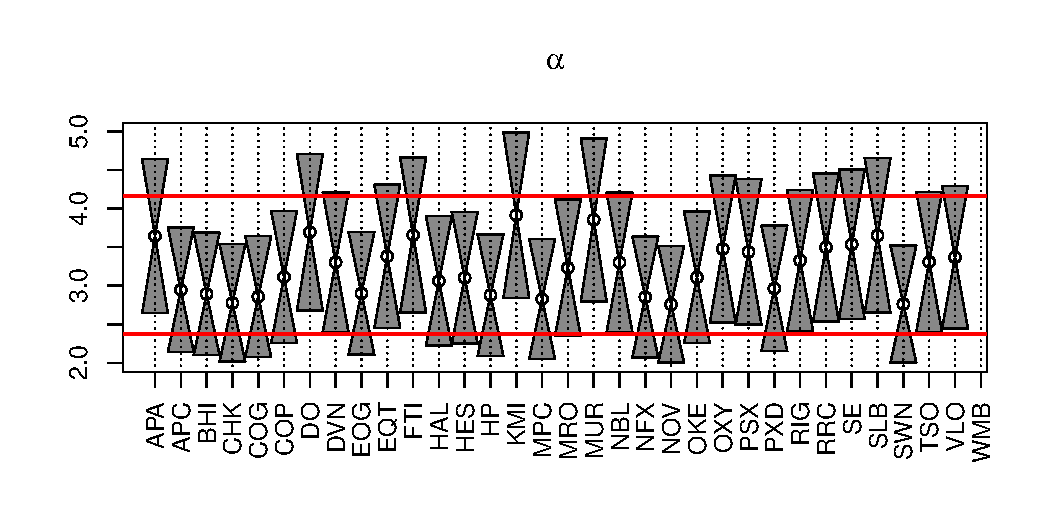
\includegraphics[width=\textwidth]{Energy_Hill_upper.pdf}
  \caption{Hill estimates of the upper tail indices of 32 stocks'
    daily return series in the {\it Energy} sector of Standard \& Poor
    500 index. Each circle coresponds to a Hill estimate; the grey
    triangles above and below it mark the 97.5\% and 2.5\% quantiles
    of its approximate normal distribution.
    The low and high red lines mark the median of the 2.5\% quantiles
    and median of the 97.5\% quantiles, respectively.
    The data are from {\it Yahoo Finance} and the labels on
    the horizontal axis are Yahoo symbols of the stocks. The data span
    from 2010-01-01 to 2015-01-01 and comprise $n=1304$
    observations. $k=(\ln n)^2 = 49$ upper order statistics are used
    for computing $\alpha_n$. 
  }
  \label{fig:Energy_Hill_upper}
\end{figure}

\begin{figure}[htb!]
  \centering
  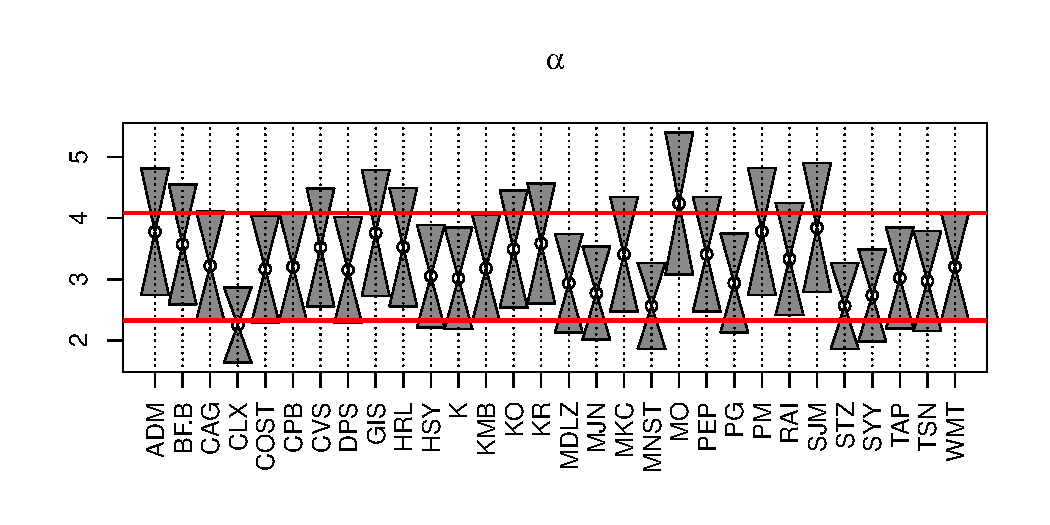
\includegraphics[width=\textwidth]{Consumer_Staples_Hill_upper.pdf}
  \caption{Hill estimates of the upper tail indices of 30 stocks'
    daily return series in the {\it Consumer Staples} sector of
    Standard \& Poor 500 index.
  }
  \label{fig:Consumer_Staples_Hill_upper}
\end{figure}

\begin{figure}[htb!]
  \centering
  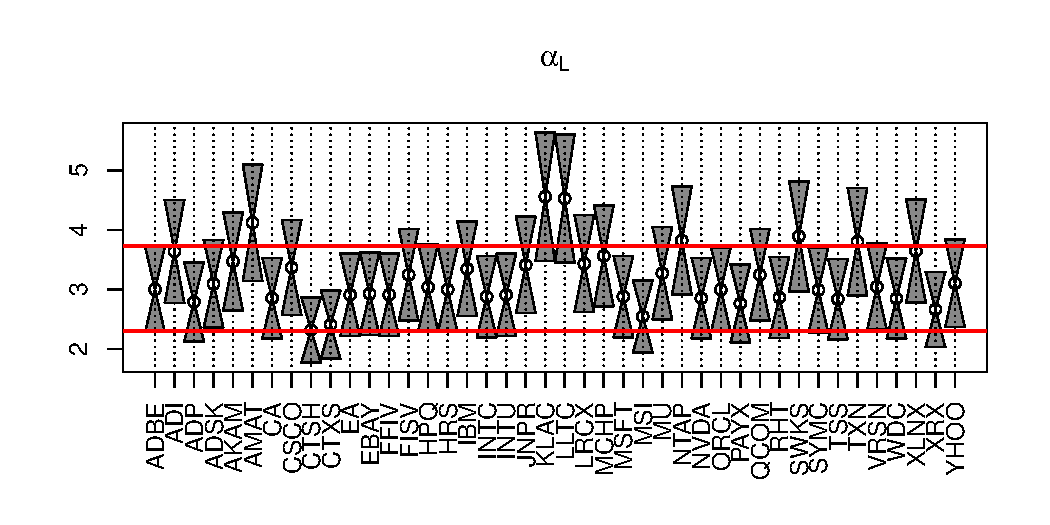
\includegraphics[width=\textwidth]{Information_Technology_lower.pdf}
  \caption{Hill estimates of the lower-tail indices of 42 stocks' daily
    return series in the {\it Information Technology} sector of S\&P
    500 index.
  }
  \label{fig:Information_Technology_lower}
\end{figure}

\section{Hybrid estimation of the assumed distribution function}
We adopt a hybrid procedure to estimate the parameters of the
distribution function assumed in eq.\eqref{eq:X_distr}: First we
obtain a Hill estimate of the lower- and upper-tail indices of an
equity return and fix $\alpha$ and $\beta$ in \eqref{eq:X_distr}
to their Hill estimates. Then we estimate $K$ and $K'$ by maximizing
the likelihood function with fixed $\alpha$ and $\beta$.

\section{Pickand's Estimator}
Pickands (1975) \cite{pickands1975statistical} proposed a different
approach to estimate the tail index than that of Hill. Assume
$\{x_i\}_{i=1}^n$ are samples from the distribution of $X$ and let $U(t)$
denote the quantile of $1 - 1/t$ of this distribution, i.e.
\[
P(X > U(t)) = {1 \over t}
\]
The key idea of Pickands' estimator is to observe
\[
\lim_{t \to \infty} {
  U(c(t) t) - U(t)
  \over
  U(t) - U(t/c(t))
} = 2^{1/\alpha}
\]
for any function $c(t)$ satisfying $c(t) \to 2$ as $t \to \infty$.
Pickands formulated the estimation problem in terms of the extreme
value index $\xi$, which is the reciprocal of the tail index $\alpha$
when the distribution of $X$ is regularly varying (cf. Embrechtsm,
Kl\"uppelberg and Mikosch \cite{Embrechts1997}).

Building upon the aforementioned observation and taking $c(t)$ to
be simply constant 2, Pickands proposed the following estimator for
$\xi$:
\[
\hat \xi = {1 \over \ln 2} \ln {
  x_{(k)} - x_{(2k)}
  \over
  x_{(2k)} - x_{(4k)}
}
\]
Dekkers and de Haan (1989) later showed \cite{dekkers1989estimation}
that Pickands' estimator was consistent in both the weak and the strong
sense, when the sequence $k(n)$ was chosen appropriately:
\begin{itemize}
\item if $k \to \infty$ and $k/n \to 0$ as $n \to \infty$,
  \[
  \hat \xi \overset{P}{\to} \xi
  \]
\item if $k \to \infty$, $k/n \to 0$ and $k / \ln(\ln n) \to \infty$
  as $n \to \infty$,
  \[
  \hat \xi \overset{a.s.}{\to} \xi
  \]
\end{itemize}
Dekkers and de Haan \cite{dekkers1989estimation} also showed the
asymptotic normality of the estimator, when some
extra technical conditions were satisfied by
$U(\cdot)$ and $k(n) \to \infty$ yet grew sufficiently slowly, i.e.
\[
\sqrt k (\hat \xi - \xi) \overset{d}{\to} N(0, v(\xi))
\]
where
\[
v(\xi) = {
  \xi^2 (2^{2 \xi + 1} + 1)
  \over
  [2 \ln(2) (2^\xi - 1)]^2
}
\]


%% \section{Hoga Test}
%% TODO: Show the test statistics of Hoga test applied to a sequence of
%% two concatenated return series. A changes in the scale is characterized
%% by a smooth bump in the test statistics while a change in the tail
%% index is characterized by a jump. Derive a theoretical result to
%% support this?

%% What is the probability of rejecting the null hypothesis when the test
%% is applied to $(X_1, X_2)$ where $X_1$ and $X_2$ have tail indices
%% $\kappa_1 \neq \kappa_2$? The probability of wrongly rejecting the
%% null hypothesis must be lower than $\alpha$.
\textcolor{red}{Review the test of Hoga}

\section{Data Analysis} \label{sec:data_analysis}
\subsection{Tail index and scale parameter}
In this section we apply the statistical tools reviewed in the
previous sections to real stock return series, denoted $X_t$
hereafter. We are interested in finding out the tail indices and the
scale parameters of the stationary distribution of $|X_t|$.

%% \subsubsection{The Energy and the Consumer Staples sectors of S\&P 500}
%% Figure \ref{fig:Energy_Hill_upper} shows the Hill estimates of the
%% tail indices of 32 stocks in the {\it Energy} sector of S\&P 500
%% index; figure \ref{fig:Consumer_Staples_Hill_upper} shows the same of
%% the {\it Consumer Staples} sector.
%% \begin{figure}[htb!]
%%   \centering
%%   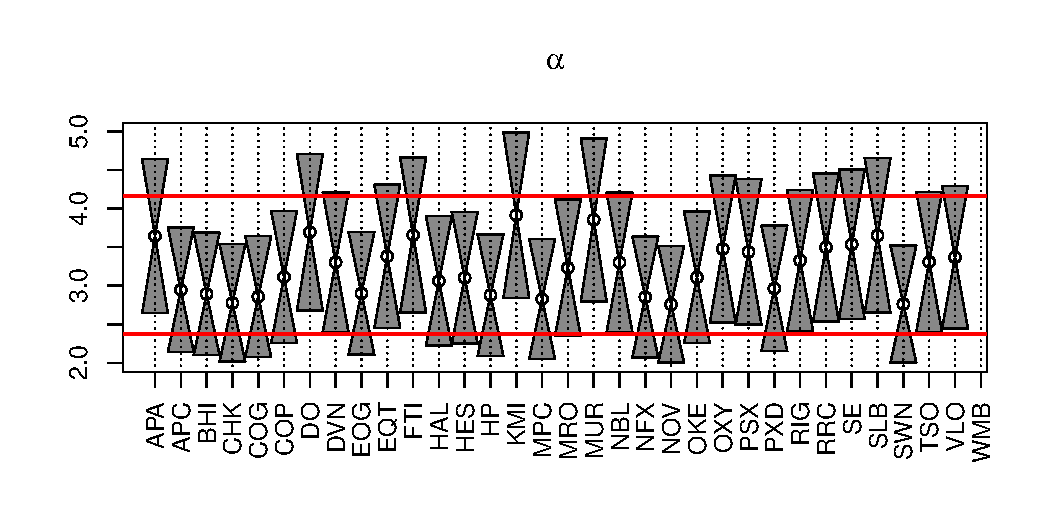
\includegraphics[width=\textwidth]{Energy_Hill_upper.pdf}
%%   \caption{Hill estimates of the upper tail indices of 32 stocks'
%%     daily return series in the {\it Energy} sector of Standard \& Poor
%%     500 index. Each circle coresponds to a Hill estimate; the grey
%%     triangles above and below it mark the 97.5\% and 2.5\% quantiles
%%     of its approximate normal distribution.
%%     The low and high red lines mark the median of the 2.5\% quantiles
%%     and median of the 97.5\% quantiles, respectively.
%%     The data are from {\it Yahoo Finance} and the labels on
%%     the horizontal axis are Yahoo symbols of the stocks. The data span
%%     from 2010-01-01 to 2015-01-01 and comprise $n=1304$
%%     observations. $k=(\ln n)^2 = 49$ upper order statistics are used
%%     for computing $\alpha_n$. 
%%   }
%%   \label{fig:Energy_Hill_upper}
%% \end{figure}

%% \begin{figure}[htb!]
%%   \centering
%%   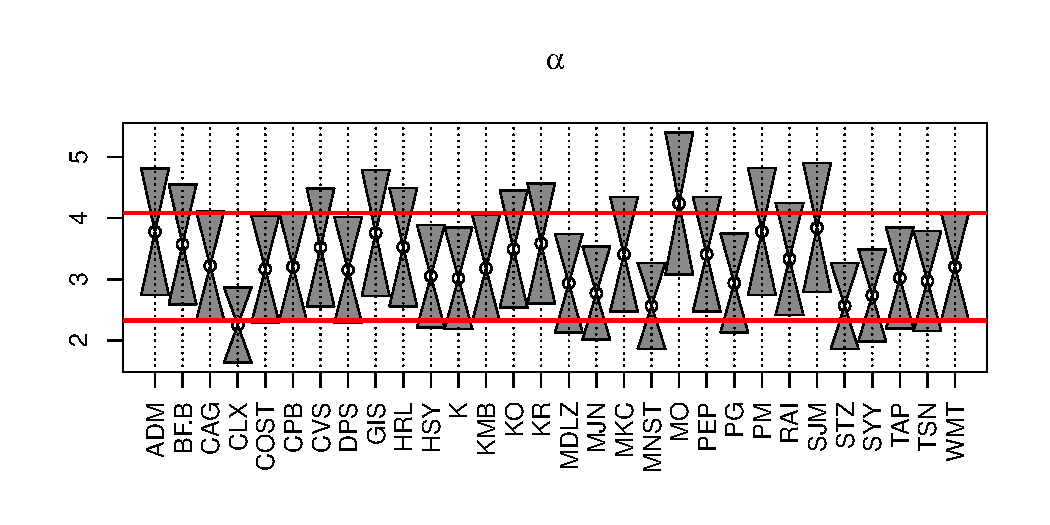
\includegraphics[width=\textwidth]{Consumer_Staples_Hill_upper.pdf}
%%   \caption{Hill estimates of the upper tail indices of 30 stocks'
%%     daily return series in the {\it Consumer Staples} sector of
%%     Standard \& Poor 500 index.
%%   }
%%   \label{fig:Consumer_Staples_Hill_upper}
%% \end{figure}

%% For our purpose, we have excluded a few stocks, though:
%% \begin{figure}[htb!]
%%   \centering
%%   \begin{subfigure}{0.45\textwidth}
%%     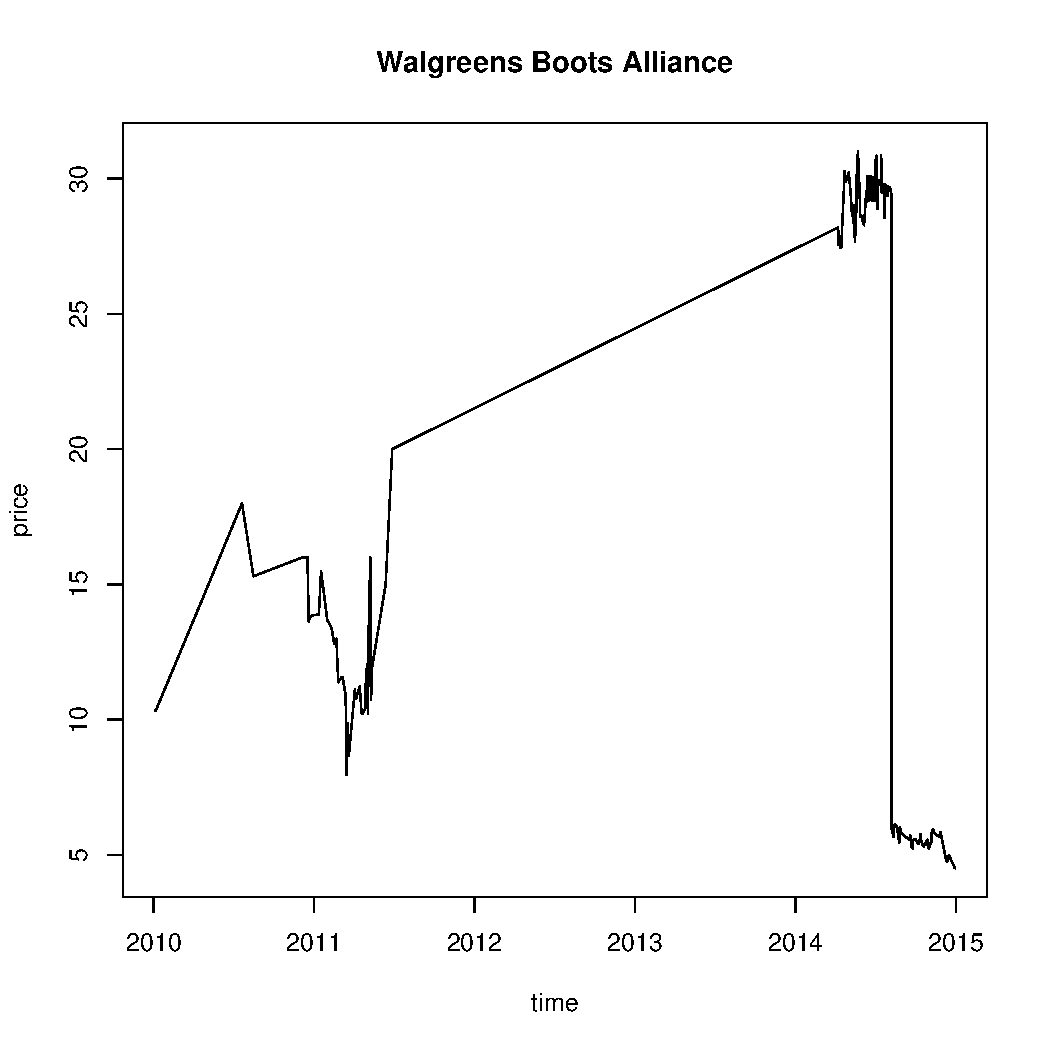
\includegraphics[width=\textwidth]{WBA_price.pdf}
%%     \caption{{\it Walgreens Boots Alliance} prices}
%%     \label{fig:EBA_prices}
%%   \end{subfigure}
%%   \begin{subfigure}{0.45\textwidth}
%%     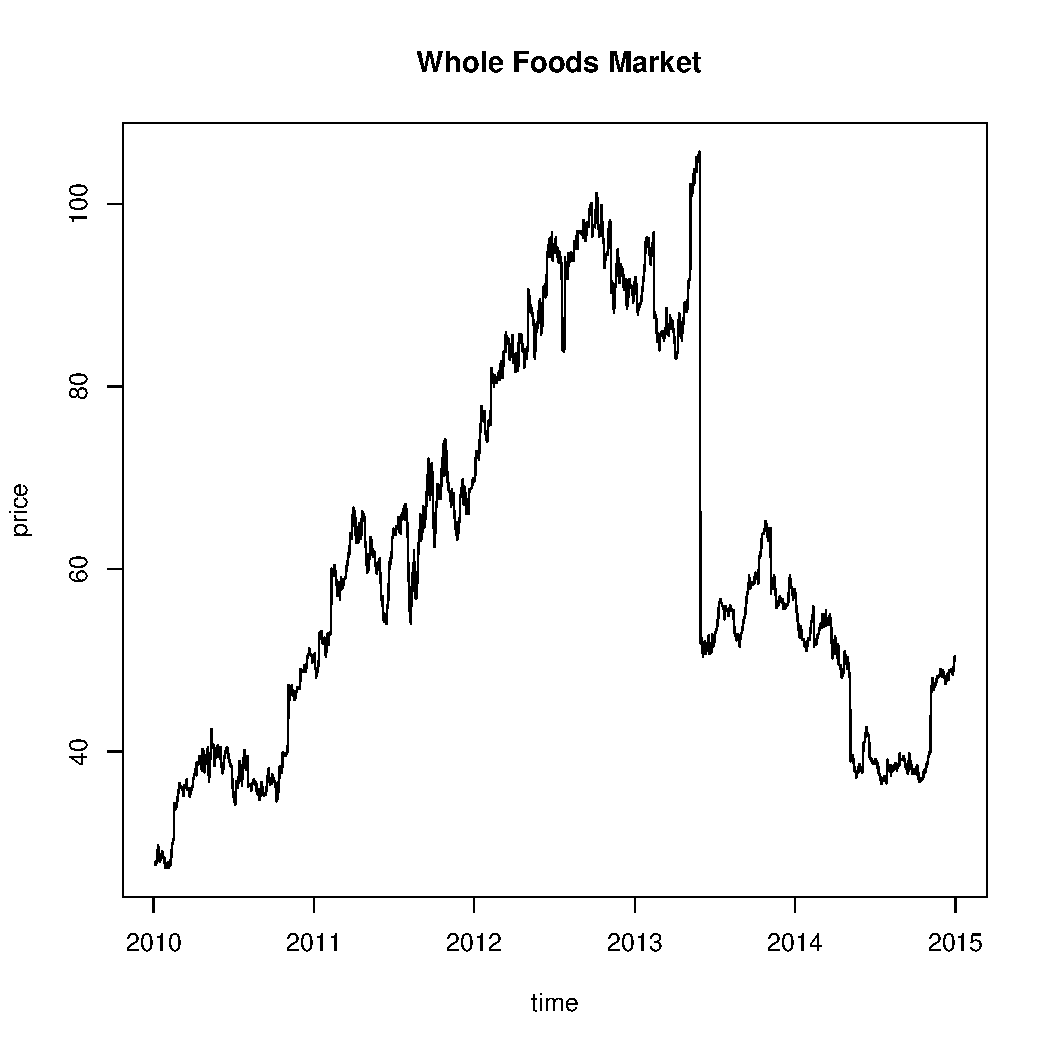
\includegraphics[width=\textwidth]{WFM_price.pdf}
%%     \caption{{\it Whole Foods Market} prices}
%%     \label{fig:WFM_prices}
%%   \end{subfigure}
%%   \begin{subfigure}{0.45\textwidth}
%%     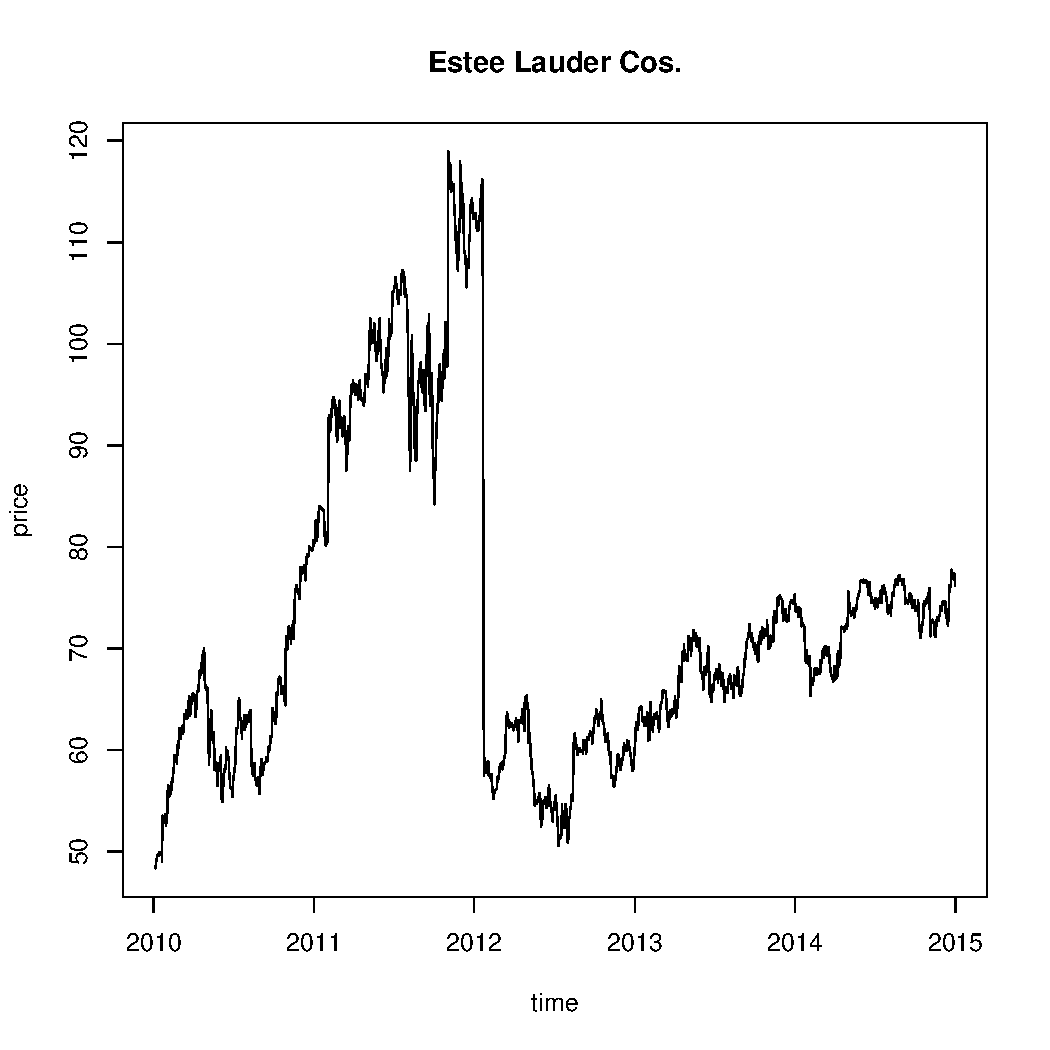
\includegraphics[width=\textwidth]{EL_price.pdf}
%%     \caption{{\it Estee Lauder Cos.} prices}    
%%     \label{fig:EL_prices}
%%   \end{subfigure}
%%   \begin{subfigure}{0.45\textwidth}
%%     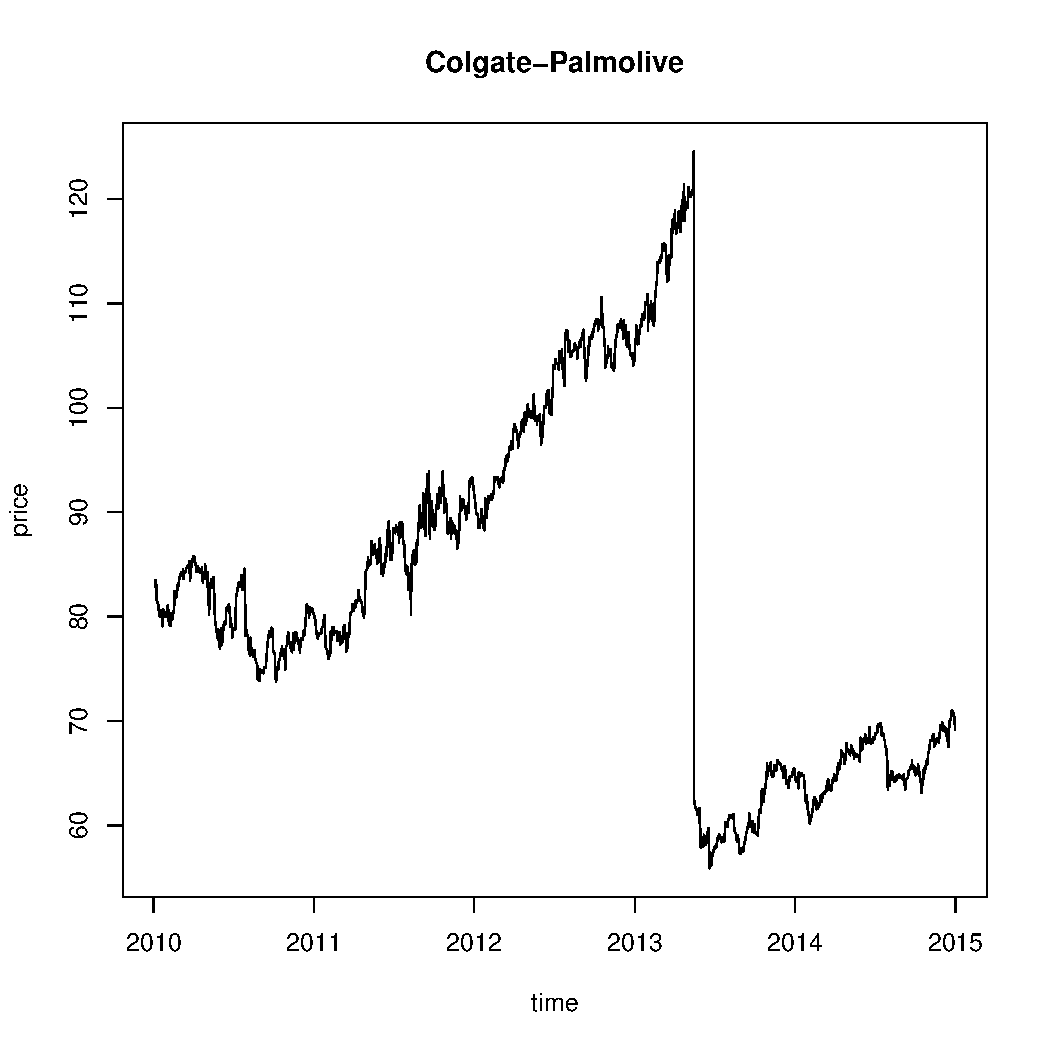
\includegraphics[width=\textwidth]{CL_price.pdf}
%%     \caption{{\it Colgate-Palmolive} prices}    
%%     \label{fig:CL_prices}
%%   \end{subfigure}
%%   \caption{Plot of prices of {\it Consumer Staples} stocks
%%     excluded from Hill estimates}
%% \end{figure}

%% \begin{itemize}
%% \item {\it Walgreens Boots Alliance}:

%%   As shown in figure (\ref{fig:EBA_prices}),
%%   this stock was traded only in a small fraction of the bank
%%   days and it is hence no surprise that the price varied
%%   tremendously.
%% \item {\it Whole Foods Market}, {\it Estee Lauder Cos.} and {\it
%%   Colgate-Palmolive}
  
%%   As seen in figures (\ref{fig:WFM_prices}), (\ref{fig:EL_prices}) and
%%   (\ref{fig:CL_prices}),
%%   the prices of these stocks were reduced by half during the
%%   period under consideration. But the price changes are the
%%   result of emission of new shares rather than random fluctuations.
%% \end{itemize}

%% Figure \ref{fig:Energy_Hill_upper} and
%% \ref{fig:Consumer_Staples_Hill_upper}
%% are suggestive of the conclusion that excluding price
%% movements due to deterministic events, tail indices of stock return
%% series tend to have the same value, within a reasonable confidence
%% interval.

%% If we look instead at the scales, differences among the stock return
%% series are however rather large. Figure (\ref{fig:Energy_Hill_Scales})
%% and (\ref{fig:Consumer_Staples_Hill_Scales}) show the Hill estimates of
%% the scale parameters of the stocks in the S\&P 500 {\it Energy} and
%% {\it Consumer Staples} sectors, respectively.
%% \begin{figure}[htb!]
%%   \begin{subfigure}{0.45\textwidth}
%%     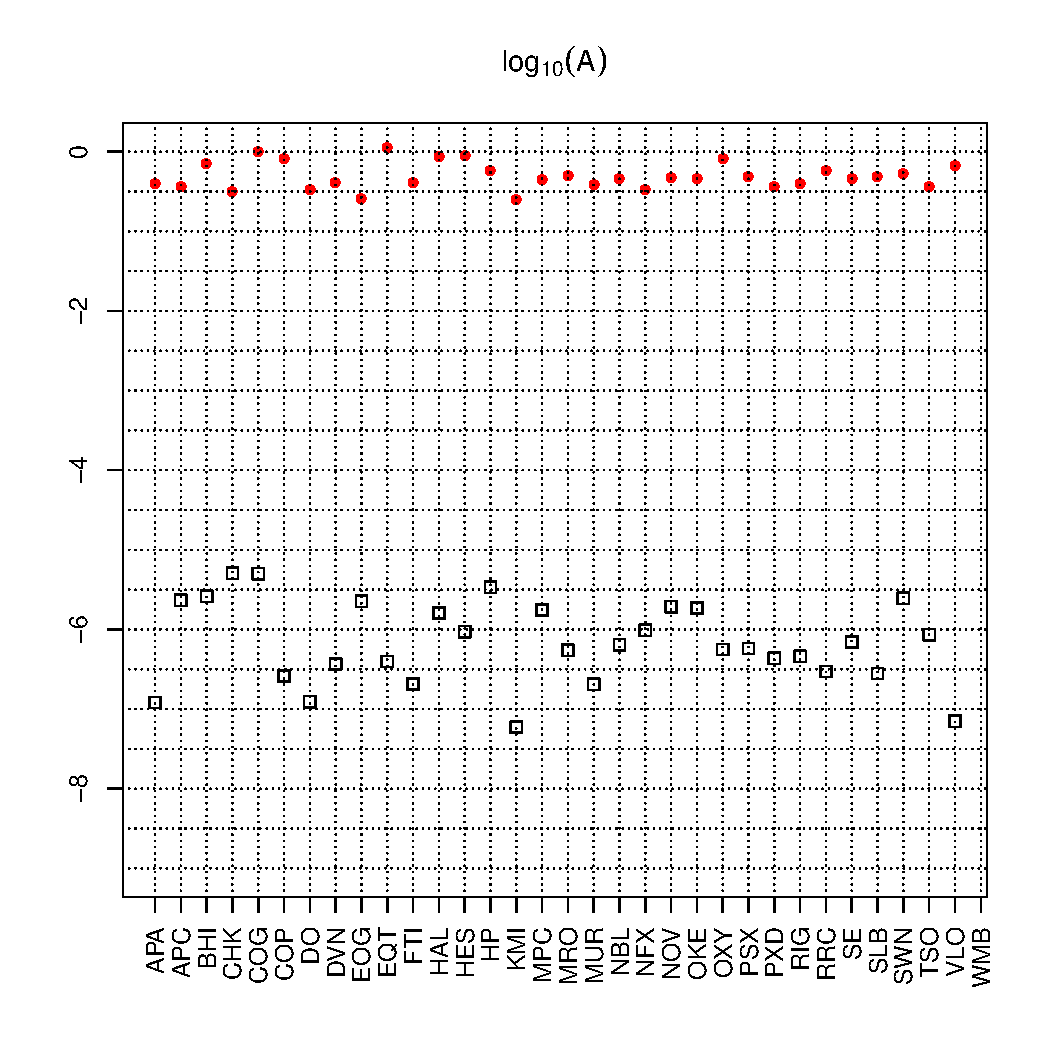
\includegraphics[width=\textwidth]{Energy_Hill_scales.pdf}
%%     \caption{{\it Energy} scale estimates}    
%%     \label{fig:Energy_Hill_Scales}
%%   \end{subfigure}
%%   \begin{subfigure}{0.45\textwidth}
%%     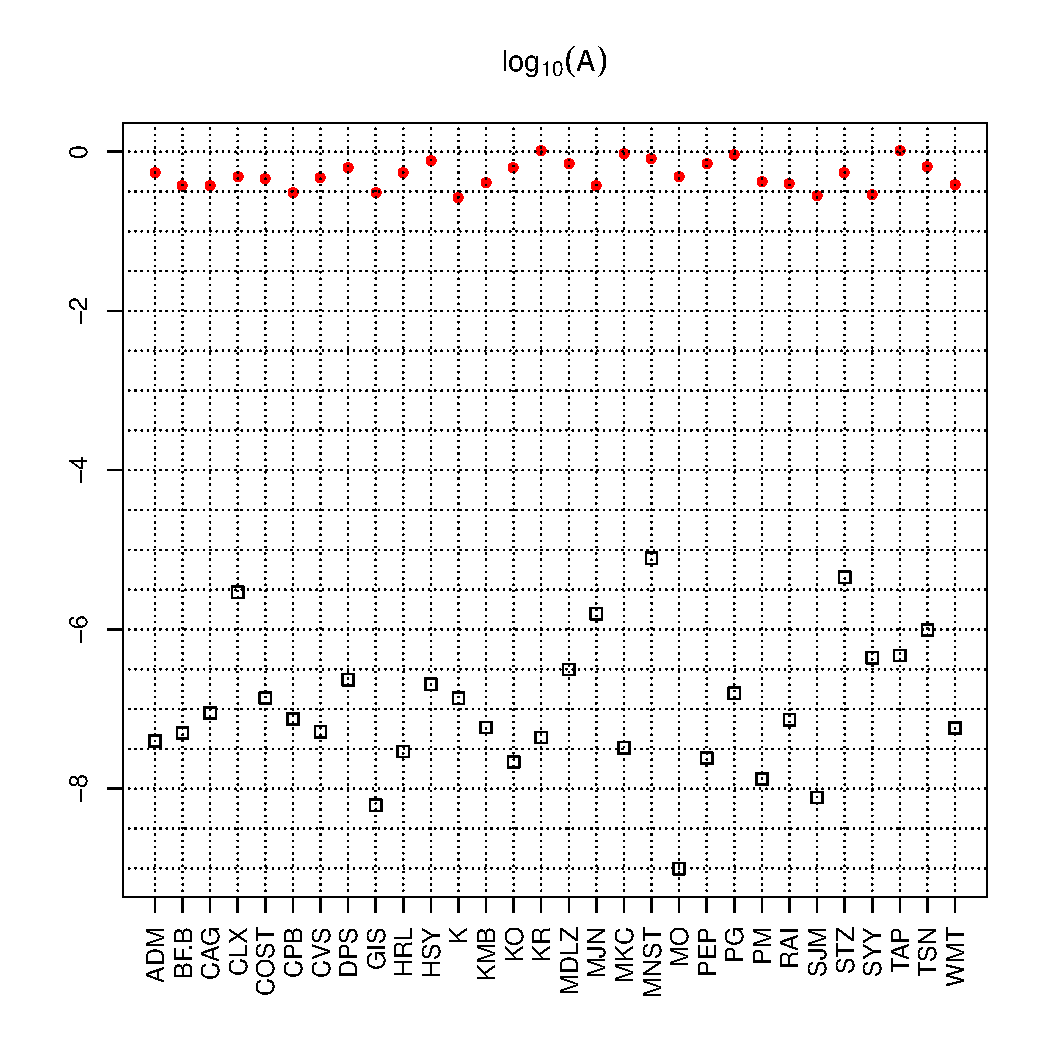
\includegraphics[width=\textwidth]{Consumer_Staples_Hill_scales.pdf}
%%     \caption{{\it Consumer Staples} scale estimates}    
%%     \label{fig:Consumer_Staples_Hill_Scales}
%%   \end{subfigure}
%%   \caption{Black boxes are Hill estimates of the scale parameters of
%%     the stock return series, while red circles are the scale estimates
%%     of simulated iid. Student's $t$ series with a degree of freedom
%%     equal to the mean value of the estimated tail indices of the stock
%%     return series. The estimates of the Student's $t$ series are
%%     included for comparison with those of the return series.}
%% \end{figure}
%% Clearly the estimated scale parameters can differ by several orders of
%% magnitude. 

%% Using the ``Peaks over Threshold'' method and the mean excess
%% function, we also obtain estimates for the tail index ($\alpha$), the
%% scale parameter ($A$) and the shift parameter ($a$) for stocks in the
%% {\it Energy} and the {\it Consumer Staples} sectors of the S\&P 500
%% index. The results are plotted in figure
%% \ref{fig:Energy_OLS_estimates} and
%% \ref{fig:Consumer_Staples_OLS_estimates},
%% respectively.
%% \begin{figure}[htb!]
%%   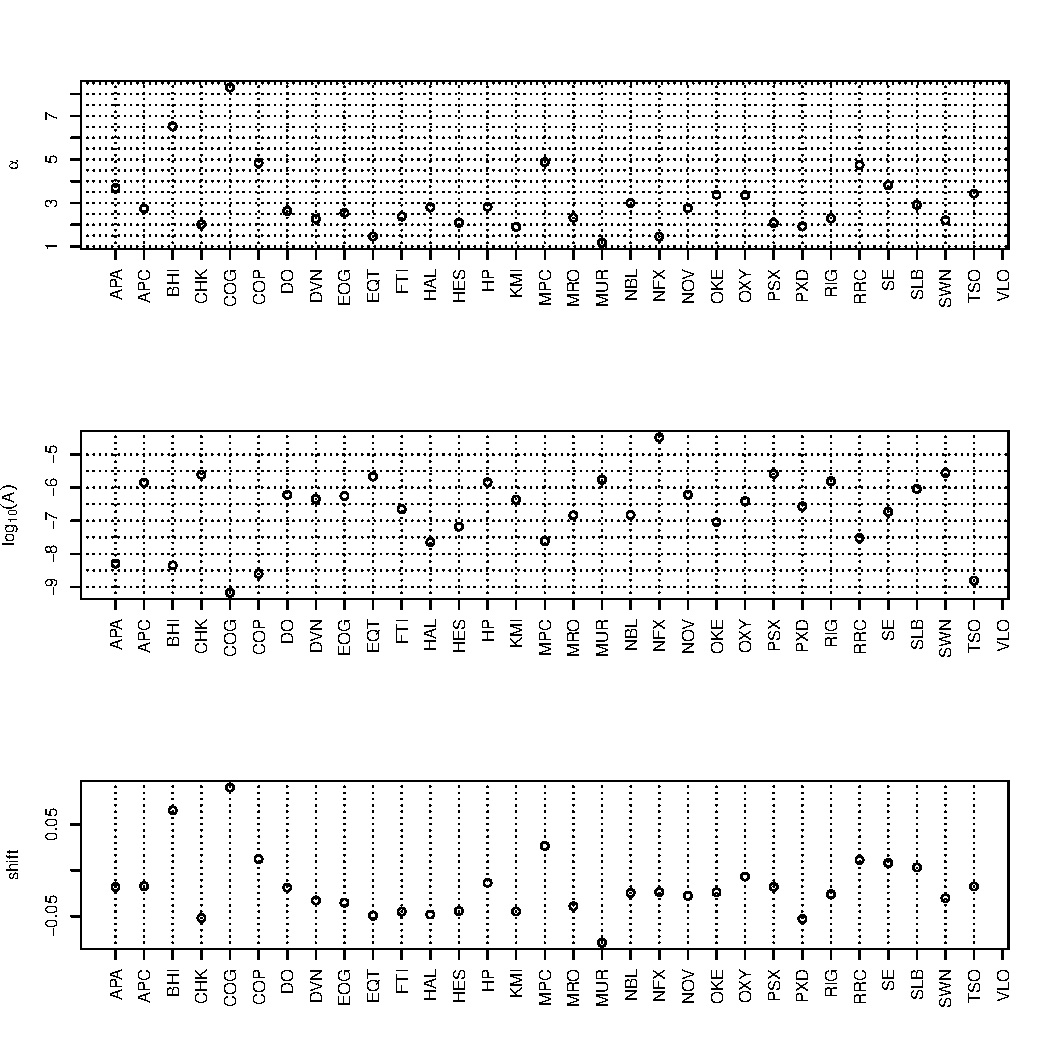
\includegraphics[width=\textwidth]{Energy_OLS_estimates.pdf}
%%   \caption{Tail parameter estimates of {\it Energy} stocks. The top
%%     plot shows the tail index estimates, the middle plot shows the
%%     10-based logarithm of the scale estimates and bottom plot shows
%%     the estimates of the shift parameter.
%%   }
%%   \label{fig:Energy_OLS_estimates}
%% \end{figure}

%% \begin{figure}[htb!]
%%   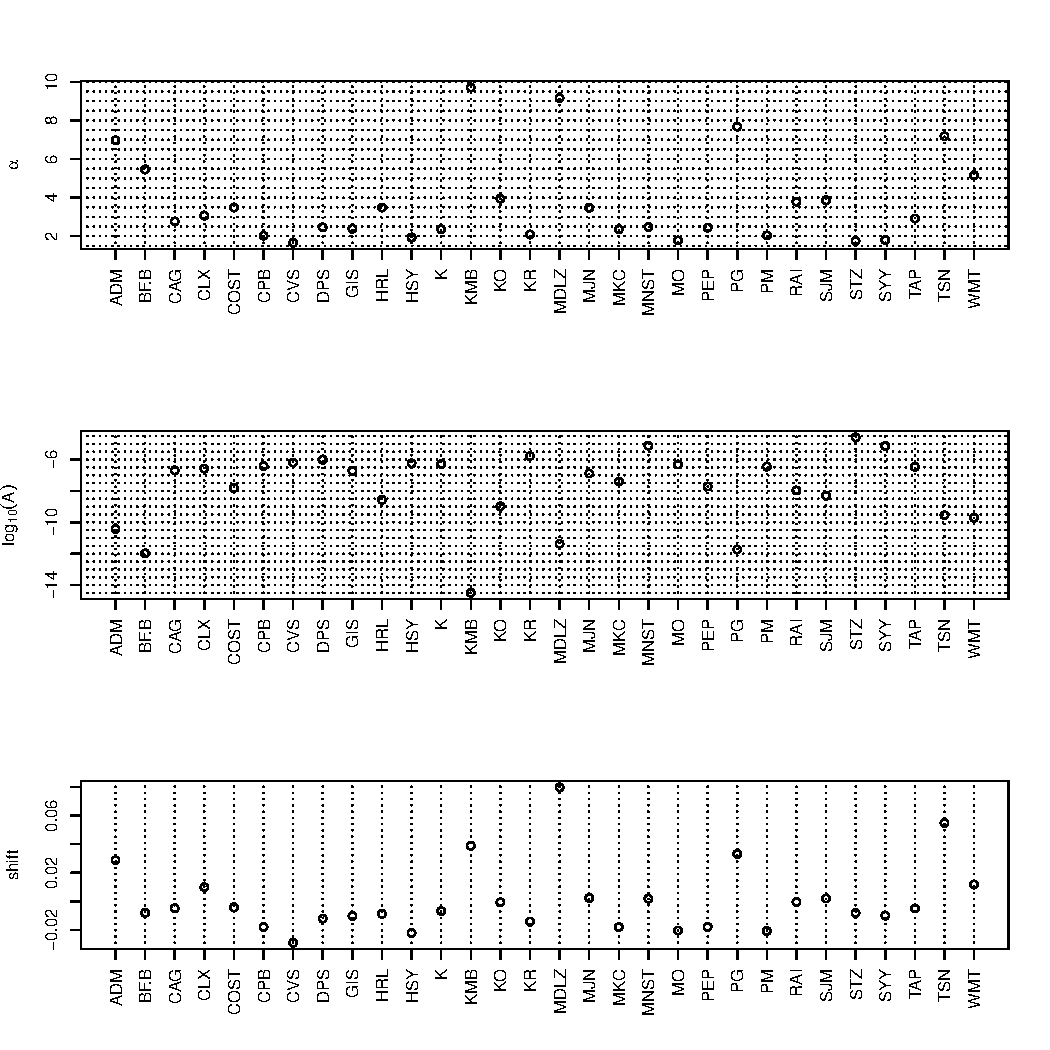
\includegraphics[width=\textwidth]{Consumer_Staples_OLS_estimates.pdf}
%%   \caption{Tail parameter estimates of {\it Consumer Staples}
%%     stocks. The top 
%%     plot shows the tail index estimates, the middle plot shows the
%%     10-based logarithm of the scale estimates and bottom plot shows
%%     the estimates of the shift parameter.
%%   }
%%   \label{fig:Consumer_Staples_OLS_estimates}
%% \end{figure}

Using Pickands' estimator, the same result of very similar tail indices
is again obtained for the {\it Energy} and the {\it Consumer Staples}
sectors. Figure \ref{fig:Energy_Pickands} and
\ref{fig:Consumer_Staples_Pickands} illustrate this claim.
\begin{figure}[htb!]
  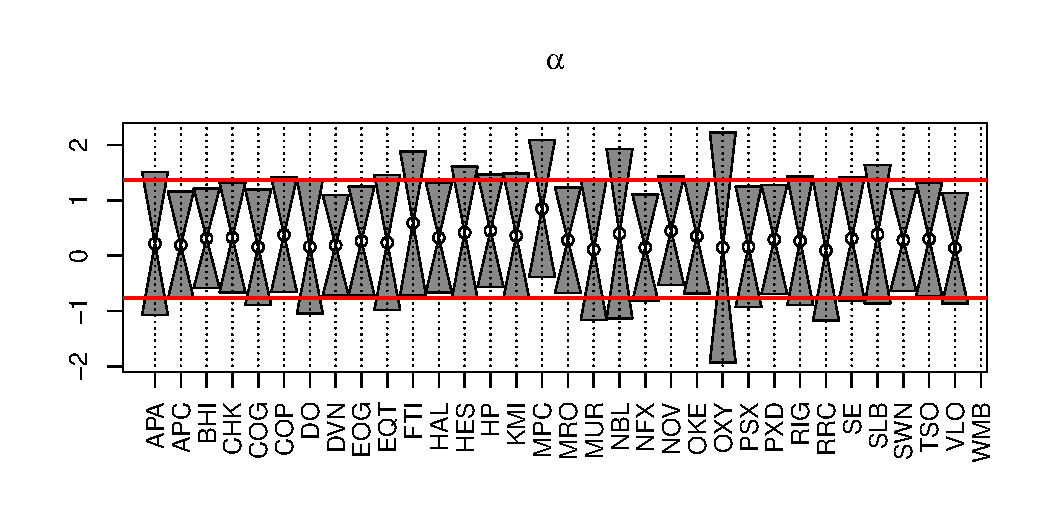
\includegraphics[width=\textwidth]{Energy_Pickands.pdf}
  \caption{Pickands' estimates of {\it Energy} stocks.}
  \label{fig:Energy_Pickands}
\end{figure}

\begin{figure}[htb!]
  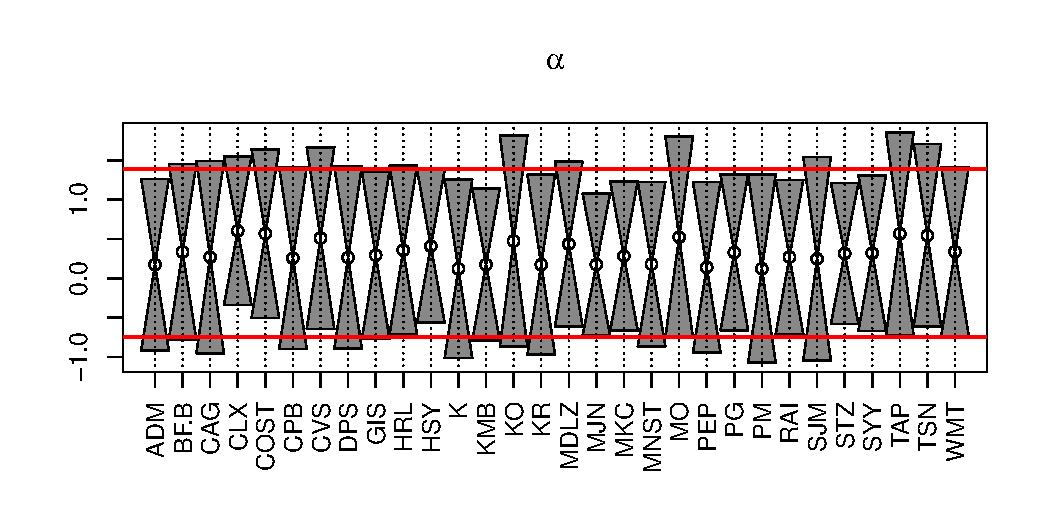
\includegraphics[width=\textwidth]{Consumer_Staples_Pickands.pdf}
  \caption{Pickands' estimates of {\it Consumer Staples} stocks.}
  \label{fig:Consumer_Staples_Pickands}
\end{figure}

%% \subsubsection{The Information Technology sector of S\&P 500}
%% Compared with the sectors of energy and consumer staples, which enjoy
%% a relatively stable demand on their products, companies of information
%% technology are more subject to volatile demand and competition. As a
%% result, one can expect their stock prices to be more volatile, implying
%% lower tail indices and larger differences between the tail indices of
%% different companies. In this section we investigate how these companies
%% differ in terms of their tail indices and scale parameters.

%% Figure \ref{fig:Information_Technology_Hill} shows the Hill
%% estimates of 42 stocks in the {\it Information Technology} sector. Daily
%% closing prices of these stocks have been available since 2000-01-01 and
%% earlier.
%% \begin{figure}[htb!]
%%   \centering
%%   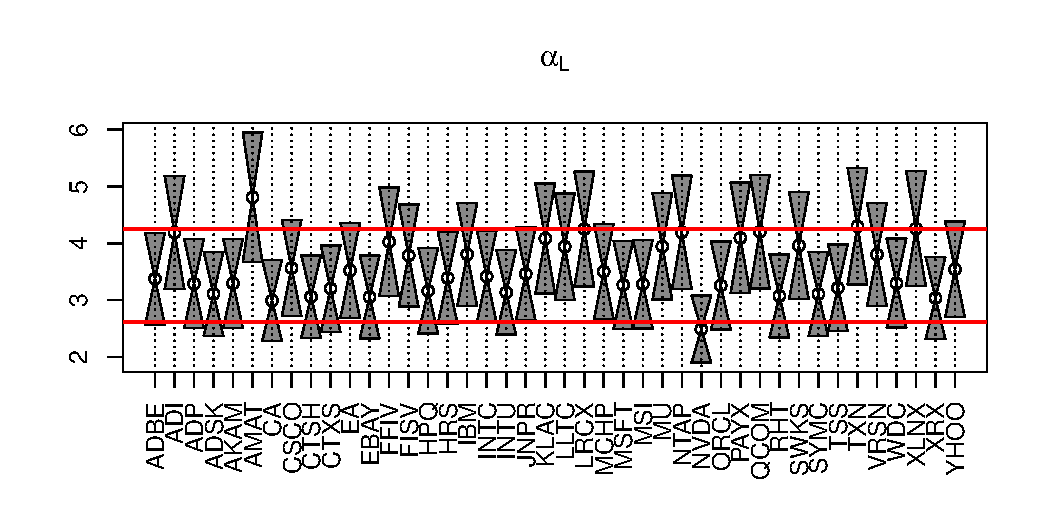
\includegraphics[width=\textwidth]{Information_Technology_Hill.pdf}
%%   \caption{Hill estimates of the tail indices of 42 stocks' daily
%%     return series in the {\it Information Technology} sector of Standard
%%     \& Poor 500 index.
%%   }
%%   \label{fig:Information_Technology_Hill}
%% \end{figure}
%% It is seen in the figure that most of the estimates fall within the
%% interval spanned by the confidence bands. Thus, given the estimation
%% precision, these are consistent with the similarity conclusion of 
%% \S\ref{sec:GDA}.

%% From the figure it appears a few pairs of stocks do have rather different
%% tail indices, e.g. ``ADI'', ``PAYX'' and ``XLNX'' versus ``CTSH'' and
%% ``NVDA''.


%% To gain more insight into these pairs, we concatenate the
%% squared return series of each pair and apply Hoga's test to the concatenated
%% sequence. Table \ref{tab:Information_Technology_Hoga} shows the test
%% statistic of each concatenated pair.
%% \begin{table}[htb!]
%%   \centering
%%   \begin{tabular}{c|c|c}
%%     \multicolumn{2}{c}{Stock(s)} & Hoga Test Statistic \\
%%     \hline
%%     ADI & CTSH & 15.52 \\
%%     ADI & NVDA & 4.726 \\
%%     PAYX & CTSH & 231.5 \\
%%     PAYX & NVDA & 110.6 \\
%%     XLNX & CTSH & 503.5 \\
%%     XLNX & NVDA & 146.5
%%   \end{tabular}
%%   \caption{Hoga Test statistic of pairs of stocks from the
%%     {\it Information Technology} sector of S\&P 500 index.
%%     The critical value at 95\% confidence level is 166.4}
%%   \label{tab:Information_Technology_Hoga}
%% \end{table}

%% \subsection{Temporal changes of the parameters}




%% Thomas: Try fitting data to a Burr distribution.
%% TODO: use GPD and POT to estimate the scale and tail index.
%% TODO: plot the Hill estimator instead of its inverse. The asymptotic
%% normal distribution of Hill estimator is found in ``Modeling Extremal
%% events''.


%% TODO: Does the scale estimator also have a convergence result from
%% which confidence bands can be derived?

%% TODO: Why does the Quintos Fan test almost always reject the null?

%% Hill (1975) \cite{hill1975simple} also proposed an estimator for the
%% scale parameter $A$:
%% \[
%% A_n = {k \over n}X_{(k+1)}^{\alpha_n}
%% \]



%% Review of CCC by Starica and others.
%% explain that the model implies that all series have the same tail index
%% Explain that economic arguments also lead to the same tail index

%% Explain that the tail functions of different series are
%% differentiated more by the scale parameter.

\section{Conclusion}
TODO: Summarize and conclude that all correlated series share the same
tail index; their tail functions differ from each other via their
scale parameters.

\bibliographystyle{unsrt}
\bibliography{../../thesis/econophysics}
\end{document}
